%!TEX root = ../thesis.tex
\chapter{Methodology}
\label{ch:methodology}
\begin{figure}[htbp]
    \centering
    \includesvg[width=\textwidth]{images/Ablaufdiagramm_white}
    \caption[Flowchart for workflow]{Flowchart for workflow. Source: own representation}
    \label{fig:Flowchart}
\end{figure}

\todo{Verweis auf Github Repo noch erwähnen?}
\todo{muss noch irgendwo das Ergebnis des DOTA Trainings erwähnt werden?}
% \begin{itemize}
%     \item Methods und Implementierung zusammenlegen
%     \item Mein Vorschlag neuer Reihenfolge
%     \item 4.3 Database
%     \item 4.2 YOLOv9
%     \item 5.3 Python Packages
%     \item 5.1 Preproc
%     \item 4.1 (Herausforderungen Preproc)
%     \item 6.1 Results 5 Folds Cross Validation
%     \item 4.4 Palma
%     \item 5.2 Bash Scripte
%     \item 
% \end{itemize}
% \todo{vollständig diesen Absatz überarbeiten}



% Die methodische Vorgehensweise dieser Arbeit ist im zugehörigen Flowchart dargestellt\todo{Referenz zum Flowchart einfügen}. Als Datengrundlage dient das \acrshort{VEDAI}-Datenset, auf dessen Basis zunächst eine Entscheidung zwischen axis-aligned und oriented Bounding Boxes getroffen wird. Da aktuelle Versionen des \acrshort{YOLO}-Frameworks grundsätzlich mit beiden Formaten umgehen können, erfolgt die Auswahl anhand ihrer jeweiligen Eignung für die Aufgaben der Objekterkennung und -lokalisierung.

% Im Anschluss wird der \Acrfull{DOTA} genutzt, um ein vortrainiertes Modell zu erzeugen, das als Ausgangspunkt für das Training mit Kanalpermutationen dient. Abhängig von der zuvor gewählten Bounding-Box-Variante wird auch die Channel Permutation mit diesem Format durchgeführt.

% Im Rahmen der Experimente werden verschiedene Kanalpermutationen (s. Tab. \ref{tab:perm}) getestet.


Die methodische Vorgehensweise dieser Arbeit ist im zugehörigen Flowchart (s. Fig. \ref{fig:Flowchart}) dargestellt. Im folgenden Abschnitt wird die Methodik dieser Arbeit beschrieben. Zunächst wird die Datengrundlage anhand der verwendeten Datensätze erläutert. Darauf aufbauend werden die eingesetzten \acrshort{YOLO}-Versionen vorgestellt. Im Anschluss folgt die Implementierung, bestehend aus den verwendeten Python-Packages sowie einer Beschreibung des Programmcodes. Danach werden die zentralen Herausforderungen im Preprocessing dargestellt. Anschließend werden die Ergebnisse der 6-Fold-Cross-Validation präsentiert, wobei eigene Folds erstellt wurden, die für alle Experimente mit \acrshort{abb}, \acrshort{obb} sowie den Permutationen (s. Tab. \ref{tab:perm}) genutzt wurden. Abschließend wird die Hardware beschrieben, auf der die Experimente durchgeführt wurden, nämlich das \acrlong{HPC} \acrshort{PALMA}, sowie die dort ausgeführten Bash-Skripte mit den für \acrshort{YOLO} verwendeten Hyperparametern.  

% \begin{itemize}
%     \item Im folgenden Abschbnitt wird die Methodik beschrieben
%     \item Erst wird die Datengrundlage anhand der verwendeten Datensätze erläutert
%     \item Dann die genutzten \acrshort{YOLO} Versionen
%     \item dann die Implementierung in Form der genutzten Python Packages und einer Beschreibung des Programmcodes
%     \item dann die Herausforderungen beim Preprocessing
%     \item dann Ergebnisse (Verteilung) der 5 Fold Cross Validation, (eigene Folds erstellt, die als für alle Experimente (\acrshort{abb} und \acrshort{obb}, sowie die Permutation genutzt wurden}))
%     \item Zuletzt die Hardware auf der die Experimente liefne (\acrlong{HPC} \acrshort{PALMA}) und die auf \acrshort{PALMA} laufenden Bash scripte mit den für \acrshort{YOLO} genutzten Hyperparametern
% \end{itemize}

\begin{table}[h!]
\centering
\begin{tabular}{l|c|c|c|c|c}
\textbf{Permutation} & \textbf{Red (R)} & \textbf{Green (G)} & \textbf{Blue (B)} & \textbf{Infrared (IR)} & \textbf{NDVI} \\
\hline
\acrshort{RGBIR}    & x & x & x & x &   \\
\acrshort{IRGB}     &   & x & x & x &   \\
\acrshort{RIRB}     & x &   & x & x &   \\
\acrshort{RGB}      & x & x & x &   &   \\
\acrshort{RGIR}     & x & x &   & x &   \\
\acrshort{RGBNDVI}  & x & x & x &   & x \\
\acrshort{GBNDVI}   &   & x & x &   & x \\
\end{tabular}
\caption{Channel permutations represented by included channels (x = channel present).}
\label{tab:perm}
\end{table}
% Die Evaluation der Ergebnisse erfolgt auf Basis der \acrshort{mAP}$_{50\text{-}95}$-Werte, welche eine standardisierte Bewertung der Modellleistung über verschiedene \Acrshort{IoU}-Schwellen hinweg ermöglichen. 

% Zuletzt wurde eine Ablationsstudie unter Verwendung der Kanäle \Acrfull{R}, \Acrfull{G}, \Acrfull{B}, \acrshort{IR} und \acrshort{NDVI} durchgeführt.

% \begin{itemize}
%     \item Im Flowchart (\todo{Ref einfügen}) ist die Methodik dieser Thesis zu erkennen
%     \item VEDAI Dataset als Grundlage; erste Entscheidung zwischen Axis Aligned und ORiented Bounding Boxen (YOLO kann mit beiden Formaten je nach VErsion umgehen, schauen welche Form besser geeignet für Objekterkennung und -detektierung ist)
%     \item dann Training des DOTA Datensatzes als Pretrained Model für die Channel Permutation
%     \item Je nach Bounding Box Evaluationsergebnis wird dann die Channel Permutation mit dieser BB Art durchgeführt. Folgende Permutationen werden berechnet: RGBIR; IRGB; RIRB; RGB, RGIR und sowie als Erweiterung optional RGBNDVI, GBNDVI
%     \item Anhand der Map50-95 Werte kann dann die Evaluation erfolgen
% \end{itemize}
\section{Database}
Die Datenbasis umfasst 2 Datensätze, die annotierte Luft- und Satellitenbildern enthalten. Das \acrshort{DOTA} Dataset wurde genutzt, um ein vortrainiertes Modell zu erzeugen, das als Ausgangspunkt für das Training mit Kanalpermutationen dient, während das \acrshort{VEDAI} Dataset mit der in Sec. \ref{sec_5Fold_CV} beschriebenen Verteilung für die Permutationsexperimente genutzt wurde.
\subsection{Vehicle Detection on Aerial Images (VEDAI) Dataset}
\label{subsec:VEDAI}

Das \Acrshort{VEDAI} Dataset \cite{vedai_web}  aus dem Jahr 2015 bietet sich als Datengrundlage an, da es hochauflösende Luftbilder enthält, die speziell für die Fahrzeugerkennung geeignet sind \cite{Razakarivony2015}. Es umfasst annotierte Daten, die Fahrzeuge in unterschiedlichen Szenarien, Größen und Orientierungen zeigen. Außerdem ist es ein Benchmark für die Detektion von sehr kleinen Objekten. Das Dataset enthält sowohl \acrshort{RGB}-Bilder als auch multispektrale Daten, was es ideal für die Untersuchung der Auswirkungen zusätzlicher Kanäle wie \acrshort{NIR} oder \acrshort{IR} auf die Objekterkennung macht. Es sind mehr als 3700 Objekte in ungefähr 1200 Bildern annotiert. Diese Objekte sind in 9 Klassen (Ship, Camping Car, Car, Pickup, Plane, Tractor, Truck, Van und Vehicles) unterteilt und der Hintergrund der Objekte ist abwechslungsreich, was die Robustheit des trainierten Modelles erhöht \cite{Razakarivony2015}. \\
Die Auflösung der Bilder liegt bei 12.5 cm \texttimes 12.5 cm pro Pixel, was ausreichend ist um einzelne Fahrzeuge zu erkennen. Die Bilder mit einer Größe von 1024 \texttimes 1024 Pixeln sind bei einer Befliegung im Jahr 2012 in US Amerikanischen Bundesstaat Utah aufgenommen worden \cite{Razakarivony2015}. 
\todo{Bsp. Bild für jede Klasse zeigen (aus Paper nehmen!; Quellenverlinkung für text und bild nicht vergessen)}



\subsection{Dataset for Objectdetection in Aerial Images (DOTA) 1.5}
\label{subsec:DOTA}

Das \Acrfull{DOTA} eignet sich aufgrund seiner Vielfalt an Klassen und seiner domänenspezifischen Ausrichtung besonders gut als Grundlage für das Pretraining in den Permutationsexperimenten. Er enthält eine große Anzahl annotierter Objekte aus verschiedenen Kategorien, die in hochauflösenden Satellitenbildern enthalten sind.

Die Bildauflösungen im \acrshort{DOTA}-Datensatz variieren stark und reichen von 800~$\times$~800 bis hin zu 20\,000~$\times$~20\,000 Pixeln. Die Datensätze umfassen sowohl \acrshort{RGB}-Bilder als auch Graustufenbilder, die den panchromatischen Kanal der GF2- und JL1-Satelliten darstellen. Die Bilder stammen aus verschiedenen Quellen, unter anderem von Google Earth und weiteren kommerziellen oder institutionellen Anbietern.

Für das Training in dieser Arbeit wurden alle 16 verfügbaren Klassen des DOTA-Datensatzes berücksichtigt. Von besonderem Interesse für die anschließenden Experimente sind jedoch die Klassen \textit{Large Vehicle}, \textit{Small Vehicle}, \textit{Plane} und \textit{Ship}, da sie eine hohe Relevanz für die Objekterkennung im urbanen bzw. infrastrukturellen Kontext besitzen.

\todo{Hinweis: Für eine bessere Anschaulichkeit sollen beispielhafte Bilder für jede Klasse aus der Originalpublikation übernommen und entsprechend mit Quellenangabe referenziert werden.}



\section{YOLOv9}
\todo{überarbeiten ist noch proposal stand; mehr auf warum und yolov9 eigenheiten eingehen, nicht basis erklären sondern das was an yolov9 geändert wurde}
Um Objekte auf hochauflösenden Satellitenbildern zu detektieren, bietet sich der "\Acrfull{YOLO}" Algorithmus an. Dieser Algorithmus, der in der Version 9 im Jahr 2024 veröffentlicht wurde \cite{yolo_v9u_github}, ermöglicht eine schnelle und präzise Objekterkennung. \acrshort{YOLO} basiert auf einer einzigen neuronalen Netzwerkarchitektur, die das Bild in Raster unterteilt und für jedes Rasterfeld Vorhersagen über die Position und Klasse von Objekten trifft. 

Die Hauptvorteile von \acrshort{YOLO} sind seine Geschwindigkeit und Genauigkeit, die es ermöglichen, große Datensätze effizient zu analysieren. Für diese Arbeit wird \acrshort{YOLO} verwendet, um Fahrzeuge auf Luftbildern zu detektieren und zu klassifizieren. Dabei könnten zusätzliche multispektrale Kanäle wie \acrshort{NIR} oder \acrshort{IR} integriert werden, um einen Vergleich zu dem reinen 3 Kanal \acrshort{RGB} Training zu ermöglichen. Die Vergleichbarkeit kann gewährleistet werden, wenn die gleichen Trainings- und Testdaten verwendet werden, bei denen der einzige Unterschied das weitere Band ist.

\subsection{YOLOv9u by Wong Kin Yiu}
\label{subsec:yolov9u}

Die Implementierung von \texttt{YOLOv9u} basiert auf der Version \texttt{YOLOv8.1.23}\cite{yolo_v9u_github} und stellt eine umfassende Weiterentwicklung der \acrshort{YOLO}-Architektur durch den Einsatz von \acrshort{PGI} und \acrshort{GELAN} dar. Neben der klassischen Objekterkennung unterstützt \texttt{YOLOv9u} zusätzliche Aufgaben wie Instanzsegmentierung, orientierte Objekterkennung, Posenabschätzung, Bildklassifikation sowie transformerbasierte Objekterkennung\cite{wang2024}. Damit bietet das Modell eine erweiterte Funktionalität gegenüber früheren \acrshort{YOLO}-Versionen, sowie der originalen \acrshort{YOLO}v9-Version, und eignet sich insbesondere für komplexe Szenarien mit mehreren Aufgabenstellungen innerhalb eines Frameworks. Diese Version wird genutzt, da sie \acrlong{obb} unterstützt.

\subsection{YOLOv9e by Ultralytics}
\label{subsec:yolov9e}

Die \texttt{YOLOv9}-Modellreihe umfasst verschiedene Varianten, die sich hinsichtlich ihrer Modellgröße, Genauigkeit und Rechenkomplexität unterscheiden. Die Bandbreite reicht dabei von der kompakten \texttt{YOLOv9t}-Variante mit einer Eingabebildgröße von $640 \times 640$ Pixeln, 2 Millionen Parametern und 7{,}7 \Acrfullpl{GFLOP} bis hin zur leistungsstärksten \texttt{YOLOv9e}-Variante mit 58{,}1 Millionen Parametern und 192{,}5 \acrshortpl{GFLOP} (siehe Tabelle~\ref{tab:yolov9-models}). 
\todo{Quelle für Tabelle einfügen}
\begin{table}[h]
\centering
\begin{tabular}{l|c|c|c|c|c} % keine äußeren vertikalen Linien
\textbf{Model} & \textbf{Image Size} & \textbf{mAP$_{\text{val}}$ 50--95} & \textbf{mAP$_{\text{val}}$ 50} & \textbf{Parameters (M)} & \textbf{FLOPs (B)} \\
\hline
YOLOv9t & 640 & 38.3 & 53.1 & 2.0 & 7.7 \\
YOLOv9s & 640 & 46.8 & 63.4 & 7.2 & 26.7 \\
YOLOv9m & 640 & 51.4 & 68.1 & 20.1 & 76.8 \\
YOLOv9c & 640 & 53.0 & 70.2 & 25.5 & 102.8 \\
YOLOv9e & 640 & 55.6 & 72.8 & 58.1 & 192.5 \\
\end{tabular}
\caption{Comparison of YOLOv9 model variants in terms of accuracy and computational complexity at an input resolution of 640$\times$640 pixels.}
\label{tab:yolov9-models}
\end{table}



Aufgrund der höchsten erzielten Genauigkeit (\acrshort{mAP}$_{\text{val}}^{50\text{-}95} = 55.6$) sowie der höchsten Rechenkapazität wurde das \texttt{YOLOv9e}-Modell für alle Experimente mit axis-aligned Bounding Boxes verwendet. Die Wahl dieses Modells erfolgte mit dem Ziel, die bestmögliche Detektionsleistung im Rahmen der Evaluierung zu gewährleisten. Diese Version wird genutzt, da sie \acrlong{abb} unterstützt.

\section{Programming Environment}
Die genutzte Programmiersprache ist Python. Die Scripte für den \acrshort{HPC} \acrshort{PALMA} wurden in Bash geschrieben.

\subsection{Python Packages}
Es wurden diverse Python Packages zur Implementatierung genutzt, die im folgenden kurz beschrieben werden. 
\subsubsection{Computer Vision 2}
Ein Teil der "Open Source Computer Vision" Bibliothek ist \Acrfull{CV2} \cite{opencv_about}. Die aktuelle Version 4.12.0 wurde am 09.07.2025 veröffentlicht \cite{opencv_release}. \\
Die Bibliothek bietet Algorithmen und Funktionen zur Bild- und Videobearbeitung an, die in dieser Arbeit hauptsächlich dazu genutzt werden, die verschiedenen Kanäle zu neuen Bildern zu kombinieren.
\subsubsection{Numpy}
Ein weiteres Open-Source Projekt ist NumPy, welches 2005 gegründet wurde, um numerische Operationen in Python zu implementieren \cite{numpy_about}. Die aktuelle Version ist 2.3.0 und wurde am 07.06.2025 veröffentlicht \cite{numpy_main_web}. \\
Mithilfe dieser Bibliothek kann eine zufällige Verteilung der Bilddaten auf die Folds realisiert werden, indem die eingelesene Bildliste einer zufälligen Permutation unterzogen wird. Darüber hinaus stellt die Bibliothek Funktionen zur Verfügung, mit denen sowohl die Berechnung und Reskalierung des \acrshort{NDVI}-Kanals als auch die Transformation der Bounding-Box-Koordinaten in das für das \acrshort{YOLO}-Framework erforderliche Format durchgeführt werden können. Zusätzlich ermöglicht sie die Umrechnung axis-aligned Bounding Boxes in oriented Bounding Boxes sowie die Flächenberechnung beider Bounding-Box-Typen.
\subsubsection{Scipy}
SciPy ist in der Version 1.16.0 am 22.06.25 veröffentlicht worden \cite{scipy-main}. Diese Bibliothek bietet Algorithmen für wissenschaftliche Berechnungen in Python an \cite{scipy-main}. Die Unterfunktion "ConvexHull" wird zur Flächenberechnung der oriented Bounding Boxen genutzt.
\todo{ab jetzt nur für analyse}
\subsection{Additional Python-Packages for data analysis}
Zur Analyse der Modelle wurden die folgenden Bibliotheken verwendet.
\subsubsection*{Matplotlib}
Die Bibliothek "Matplotlib" wurde in der Version 3.10.0 am 23.12.2024 veröffentlicht\cite{matplotlib}. Im Rahmen dieser Arbeit werden durch diese Erweiterung die Datenanalysen und die Ausgabe der Plots ermöglicht.
\subsubsection*{Seaborn}
"Searborn" ist in der Version 0.13.2 im Januar 2024 veröffentlicht worden \cite{seaborn}. Die Bibliothek ermöglicht das Erstellen von Grafiken, wie Boxplots, zur vereinfachten Datenanalyse.
\subsubsection*{pandas}
Die Bibliothek "pandas" ist ebenfalls ein Open Source Datenanalyse und -manipulierungstool. Die aktuelle Version 2.3.1 wurde am 07.07.2025 veröffentlicht. Die Bibliothek wird auch zur Datenanalyse in dieser Arbeit verwendet \cite{pandas}.

\section{Implementation Preprocessing}
\todo{weniger Funktionsnamen}
Damit die Trainingsdaten vom Deep-Learning-Modell YOLOv9 verarbeitet werden können, ist eine Vorverarbeitung notwendig, die deren Format und Struktur an die Anforderungen des Modells anpasst. Der genaue Ablauf dieser Vorverarbeitung wird im Folgenden beschrieben.
\subsection{DOTA Dataset}
Im Rahmen der Datenvorverarbeitung wurden ausschließlich die originalen Rohbilder des \acrshort{DOTA}-Datensatzes verwendet, ohne dass ein Zuschnitt oder eine anderweitige Modifikation der Bildinhalte vorgenommen wurde. Der Fokus der Verarbeitung lag auf der Umwandlung der vorhandenen Labeldaten in das \texttt{YOLOv9-OBB}-Format, welches polygonale Objektumrandungen in Form einer Punktsequenz \((x_1, y_1, x_2, y_2, \ldots)\) beschreibt (vgl. \todo{text\texttt{\textbackslash todo\{Ref zur Formatbeschreibung einfügen\}}}).

Für jedes Bild stellt \acrshort{DOTA} eine separate Textdatei bereit, die alle zugehörigen Annotationen enthält. Zu Beginn wurde eine standardisierte Ordnerstruktur nach dem \acrshort{YOLO}-Schema erstellt, bestehend aus den Unterverzeichnissen \texttt{train/images}, \texttt{train/labels}, \texttt{val/images} und \texttt{val/labels}. Die Annotationsdateien wurden daraufhin zeilenweise eingelesen und verarbeitet.

Jede Zeile, die ein einzelnes Objekt beschreibt, wurde zunächst an die jeweilige Bildgröße angepasst, wobei die absoluten Koordinaten der Objektrahmen in relative Werte normalisiert wurden. Da die Auflösung der Bilder im \acrshort{DOTA}-Datensatz stark variiert (zwischen \(800 \times 800\) und \(20{,}000 \times 20{,}000\) Pixeln), war eine dynamische Skalierung erforderlich. Die konvertierten Informationen wurden anschließend in das \texttt{YOLOv9}-Format überführt, wobei die Klassen-ID jeweils am Anfang der Zeile stand. Die so erzeugten Labeldateien wurden unter Beibehaltung des ursprünglichen Dateinamens gespeichert.

Insgesamt wurden sämtliche 16 im \acrshort{DOTA}-Datensatz enthaltenen Objektklassen berücksichtigt und entsprechend konvertiert. Die Bilddaten selbst blieben unangetastet und wurden in ihrer Originalform auf den HPC Cluster \acrshort{PALMA} übertragen. Aufgrund der hohen Anzahl an verfügbaren Annotationen gestaltete sich der Konvertierungsprozess zeitintensiv.

% \begin{itemize}
%     \item Bilder nicht zugeschnitten, Rohbilder verwendet, wie vom Dataset bereitgestellt
%     \item nur labels in yolo v9 obb format (x1,y1,x2,y2... \todo{ref zu erklärung einfügen}) konvertiert
%     \item \acrshort{DOTA} bietet für jedes Bild eine txt mit den dazugehörigen labels an
%     \item Erst wird die Ordnerstruktur (train/images, train/labels, val/images, val/labels) für die daten erstellt
%     \item diese txt wird eingelesen und dann Zeile für Zeile durchgegangen 
%     \item Jede Zeile wird konvertiert (normalisiert auf die Größe des jeweiligen Bildes, Bildgröße ist bei \acrshort{DOTA} nicht gleich sondern schwankt von 800*800 bis 20.000 * 20.000) und in das format gebracht (so das klasse vorne steht) und dann wird es in einer neuen txt gespeichert (wie bei der Originaldatei (dateiname ist gleich) nur umgewandelt ins yolo format)
%     \item alle 16 vorhandenen Klassen werden umgewandelt
%     \item letztendlich werden nur die labels konvertiert, die Bilder bleiben unangetastet und werden direkt auf PALMA hochgeladen
%     \item Menge von Labels sehr hoch, konvertierung  dauert lange
% \end{itemize}
\subsection{VEDAI Dataset}


Die Verarbeitung des \acrshort{VEDAI}-Datensatzes erfolgt über eine zentrale Hauptmethode, in der mehrere konfigurierbare Parameter in Form von booleschen Variablen bereitgestellt werden. Besonders wichtig ist hierbei der Parameter \texttt{oriented}, welcher angibt, ob die \Acrfullpl{BB} als achsenparallele Rechtecke oder als orientierte Rechtecke im \acrshort{obb}-Format generiert werden. Zusätzlich kann über \texttt{bool\_create\_yaml} gesteuert werden, ob für jedes erzeugte Trainingsset eine entsprechende \acrshort{YAML}-Datei automatisch mitgeneriert werden soll.

Ein weiterer Parameter, \texttt{merge\_ir\_bool}, ermöglicht es, das Infrarotbild (IR) in die erzeugten Bilddaten zu integrieren. Mithilfe des Parameters \texttt{namestring} lässt sich jedem erzeugten Trainingsset ein individueller Name zuweisen. Entscheidend für die Zusammensetzung der Bildkanäle ist das Dictionary \texttt{perm\_object}, in dem über boolesche Werte festgelegt wird, welche Kanäle (z.\,B. \acrshort{R}, \acrshort{G}, \acrshort{B}, \acrshort{IR}, \acrshort{NDVI}) in das finale Bild aufgenommen werden sollen.

In der zentralen Hauptfunktion wird anschließend bestimmt, welche Teilmengen des Datensatzes erzeugt werden sollen. Dies betrifft u.\,a. \texttt{ablation}-Sets, \texttt{perm}-Datasets oder \texttt{aab\_vs\_obb}-Konfigurationen. Für beide erstgenannten Varianten folgt der Ablauf einem konsistenten Schema: Die Parameter \texttt{oriented} und \texttt{merge\_ir\_bool} werden aktiviert, ein Speicherpfad für das erzeugte Dataset definiert, und das \texttt{perm\_object} wird entsprechend der gewünschten Kanalzusammenstellung konfiguriert. Beispielweise wird für die Kombination \texttt{rgir} lediglich \acrshort{R}, \acrshort{G} und \acrshort{IR} im \texttt{perm\_object} auf \texttt{true} gesetzt. Im Anschluss wird mittels einer \texttt{for}-Schleife über die Folds 0 bis 5 iteriert und für jeden Fold mit der Methode \texttt{create\_fold\_cross\_validation} das entsprechende Datenset aus Trainings-, Validierungs- und Testdaten generiert (vgl. \todo{Verweis auf entsprechende Funktion}).

\paragraph{Erzeugung von Folds via \texttt{create\_fold\_cross\_validation}}

Diese Methode übernimmt die vollständige Erstellung der Ordnerstruktur im für \acrshort{YOLO} erforderlichen Format (\texttt{train/images}, \texttt{train/labels}, \texttt{val/images}, \texttt{val/labels}, \texttt{test/images}, \texttt{test/labels}). Zudem wird eine \acrshort{YAML}-Datei erzeugt, die sowohl die Pfade zu den Bilddateien als auch die Anzahl der enthaltenen Kanäle enthält. Ein Trainingsdatensatz setzt sich stets aus drei Komponenten zusammen: 
\begin{enumerate}
    \item \textbf{Trainingsdaten:} Bestehen aus den Bildern der übrigen Folds (also alle außer dem aktuellen Fold und Fold 6).
    \item \textbf{Validierungsdaten:} Entsprechen den Bildern des jeweils aktuellen Folds.
    \item \textbf{Testdaten:} Bestehen stets aus den Bildern von Fold 6.
\end{enumerate}

Der aktuell ausgewählte Fold wird aus der Liste mit allen Folds entfernt, um Überschneidungen mit Trainings-, Validierungs- und Testdaten auszuschließen. Anschließend wird die zentrale Datei mit allen Labelinformationen des Datensatzes eingelesen. Über eine \texttt{for}-Schleife werden alle Folds durchlaufen, die nicht dem aktuellen Fold entsprechen. Dabei wird jeweils die Datei mit den Bildnamen eingelesen und für jedes dieser Bilder die Funktion \texttt{create\_image\_and\_label} aufgerufen.

Diese Funktion liest für jede Zeile das zugehörige \acrshort{RGB}- und \acrshort{IR}-Bild ein und filtert die Labels so, dass nur die zum aktuellen Bild gehörenden Annotationen weiterverarbeitet werden. Das neue Bild wird anschließend in den jeweiligen Zielpfad kopiert, wobei intern die Funktion \texttt{merge\_RGB\_IR\_image} zur Anwendung kommt. Diese Funktion stellt sicher, dass nur die im \texttt{perm\_object} spezifizierten Kanäle in die Zieldatei übernommen werden (vgl. \todo{ref einfügen}Referenz zur Funktion). Im Anschluss wird die Funktion \texttt{create\_label\_file} aufgerufen, um das zugehörige Label-File im gewünschten Format zu erzeugen (vgl. \todo{ref einfügen} Referenz zur Funktion).

Nach dem Abschluss der Verarbeitung aller Trainingsfolds wird abschließend sowohl der Validierungsfold (aktueller Fold) als auch der Testfold (immer Fold 6) mithilfe der Funktion \texttt{create\_image\_and\_label} separat verarbeitet. Nach deren erfolgreichem Durchlauf gilt das Datenset für die jeweilige Kanal-Kombination als vollständig erstellt.

\paragraph{Fusion von RGB- und IR-Bildern (\texttt{merge\_RGB\_IR\_image})}

Diese Methode lädt die entsprechenden \acrshort{RGB}- und \acrshort{IR}-Bilder und erzeugt basierend auf der Vorgabe im \texttt{perm\_object} eine kombinierte Bilddarstellung. Die Verschmelzung erfolgt mit Hilfe von \texttt{cv2.merge}. Falls gefordert, wird innerhalb dieser Funktion zusätzlich ein \acrshort{NDVI}-Bild erzeugt. Zur numerischen Stabilisierung bei der \acrshort{NDVI}-Berechnung wird der Nenner (\acrshort{IR} + \acrshort{R}) auf mindestens 0{,}01 gesetzt, um Division durch Null zu vermeiden. Die \acrshort{NDVI}-Werte werden anschließend skaliert und als 8-Bit-Bild zurückgegeben. Vor dem Zusammenführen werden die \acrshort{RGB}-Kanäle immer einzeln extrahiert. Die Funktion \texttt{copy\_image} übernimmt dann das Schreiben der erzeugten Bilder an den vorgesehenen Zielpfad.

\paragraph{Erzeugung von Label-Dateien (\texttt{create\_label\_file})}

Zur Erstellung der Label-Datei wird zunächst der Pfad zur Ausgabedatei bestimmt und das zugehörige Bild eingelesen, um die Bilddimensionen für die spätere Normalisierung zu ermitteln. Anschließend werden alle übergebenen Label-Informationen durchlaufen. Für jedes Label wird mithilfe der Funktion \texttt{get\_bounding\_box\_in\_px} die Bounding Box in Pixelkoordinaten berechnet.

Im nächsten Schritt wird die Zielzeile im \acrshort{YOLO}-Format erstellt: Die Klasse wird dabei in eine numerische \acrshort{ID} zwischen 0 und 8 überführt (mittels einer internen Mapping-Funktion), gefolgt von den acht Koordinatenpunkten der Bounding Box, jeweils durch Leerzeichen getrennt.

Im Fall von \texttt{oriented = true} werden die acht Punkte einer rotierbaren Box gespeichert. Ist \texttt{oriented = false}, können die Koordinaten entweder in klassischer \acrshort{YOLO}-Darstellung (zentrumsbasiert mit Höhe und Breite) oder als achsenparalleles Rechteck im \acrshort{obb}-Format gespeichert werden. Die Umwandlung erfolgt hier durch unterschiedliche Konvertierungsfunktionen. Abschließend wird die Zeile in die Datei geschrieben und der Prozess für das nächste Label wiederholt.

\paragraph{Berechnung der Bounding Box in Pixeln (\texttt{get\_bounding\_box\_in\_px})}

Diese Funktion dient der Extraktion und Transformation der Labelkoordinaten aus dem ursprünglichen \acrshort{DOTA}-Format. Zunächst wird der Label-String anhand von Leerzeichen in seine Bestandteile zerlegt. Die Position (x, y) sowie die Orientierung befinden sich an den Stellen 1 bis 3 des Arrays, während sich die Klassen-\acrshort{ID} an Position 12 befindet. Die Eckpunkte der Bounding Boxen (x-Werte: Positionen 4–8, y-Werte: 8–12) werden extrahiert und daraus die Seitenlängen berechnet.

Die längsten Seiten des Objekts werden identifiziert und als Fahrzeuglänge, die kürzeren als Fahrzeugbreite angenommen. Aus den längsten Seiten wird ein Richtungsvektor berechnet, und der Winkel der Fahrzeugausrichtung über den Arctan bestimmt. Die vier Eckpunkte der orientierten Box werden schließlich unter Berücksichtigung von Fahrzeugmitte, Länge, Breite und Rotationswinkel berechnet.

Ist \texttt{oriented = true}, so werden die vier Eckpunkte als ganzzahlige Koordinaten-Tupel zurückgegeben. Ist \texttt{oriented = false}, wird aus den minimalen und maximalen x- und y-Werten der rotierten Box eine achsenparallele Bounding Box erzeugt und zurückgegeben.

% \begin{itemize}
%     \item Main Methode
%     \begin{itemize}
%         \item Verschiedene Bools um Einstellungen vorzunehmen; am wichtigsten ist "oriented", für die Form der Bounding Boxen (BB) ob axis aligned oder obb
%         \item "bool\_create\_yaml" um einzustellen ob für jedes Trainingsset eine yaml direkt miterzeugt werden soll
%         \item "merge ir bool" um einzustellen ob das IR Bild mit in die erzeugten Bilder eingefügt werden soll
%         \item "namestring" um jedem Trainingsset nen individuelen Namne geben zu könne
%         \item (Wichtig) "perm object" ist ein dictionary wo festgelegt wird welche Kanäle in das Bild kommen (R,G,B,IR,NDVI), hier kann mit True und False einfach die gewünschte kombination eingefügt werden
%         \item ansonsten wird in der Funktion einfach aufgerufen welche Datensets erzeugt werden sollen (ablation,perm datasets oder aab\_vs\_obb datasets)
%         \item in diesen beiden Funktionen (perm und ablation) ist der Ablauf immer ähnlich -> oriented und merge ir bool werden auf true gesetzt und der Pfad zum Abspeichern des Datasets festgelegt. Dann wird das perm object je nach Bedarf auf True gesetzt (bspw. für rgir wird nur r, g, ir im Permobject auf true gesetzt) und dann wird mit einer for schleife von 0 bis 5 mit der Funktion "create fold cross validation" der entsprechende fold erzeugt (referenz zu Funktion einfügen?)
%     \end{itemize}
%     \item Create Fold Cross Validation
%     \begin{itemize}
%         \item Ordnerstruktur wird erstellt (wie von yolo gefordenr train/images, train/label, val/images, val/label, test/images, test/label)
%         \item yaml datei mit pfaden zu den bildern und der aktuellen anzahl an Channeln in den Bildern wrid erstellt
%         \item aktueller Fold wird aus den Folds zur Erstellugn der Trainingsdaten genommen, (keien ÜBerschneidung möglich mit Training, Val und Test)
%         \item das file mit allen labels in dem Dataset wird eingelesen
%         \item For Schleife die alle Folds, die nciht der aktuelle Fold sind, startet
%         \item das txt mit den bildernamen des jeweiligen folds wird eingelesen und die funktionsinterne Funktion "create image and label" wird aufgerufen. diese durchläuft alle Zeilen des gerade gelesenen Fold txt. die pfade für das rgb und ir bild werden festgelegt um die bilder einzulesen und danach werden die labels so gefiltert, dass nur die Labels für das aktuelle Bild noch vorhanden sind. Dann wird das neue Bild in den jeweiligen Pfad kopiert (in der "copy image" Funktion wird auch "merge RGB IR image" FUnktion genutzt, um nur die jeweilige kanalkombination an den Zielpfad zu kopieren, Referenz verlinken); dann wird die create label file funktion aufgerufen, die das jeweilige txt zu dem bild erzeugt (Referenz verlinken, wird später noch beschrieben)
%         \item dann werden die pfade den jeweiligen validierungs (aktueller fold) und den testfold (immer der 5.) festgelegt und die obig beschriebene "create image and label" funktion wird dann nochmal einzeln jeweils für den validierung und testfold aufgerufen. Wenn die beiden durchgelaufen sind ist der Datensatz für die kanalkombination fertig prozessiert
%     \end{itemize}
%     \item merge RGB and IR image
%     \begin{itemize}
%         \item lädt die entsprechenden rgb und ir bilder und gibt , je nach angabe im perm object mit der cv2 merge die entspechende kombination zruück. hier wird auch das NDVI Bild erzeugt, falls es im Permobject gefordert wird (mit calc ndvi; Nenner wird ir +r, wenn nenner 0 ist wird auf 0.01 gesetzt um numerische stabilität zu gewährliesten und Divison durch 0 zu vermeiden; NDVI = (IR-r)/Nenner; dann auf 0-255 skaliert und zurückgegeben )
%         \item rgb bild wird in jedem fall in die kanäle gesplittet bevor es gemerged und zurückgegeben wird; copy image schreibt das dann an den gegebenen Pfad, was zurückgegeben wurde
%     \end{itemize}
%     \item create Label file
%     \begin{itemize}
%         \item file path für die Zieldatei wird erstellt
%         \item jeweiliges bild wird eingelesen (um die Größe zu bekommen für die normalisierung)
%         \item alle übergebenen Labels werden mit einer for schleife iteriert, die transf label variable (verweis auf get bounding box in px Funktion) speichert die bb in pixeln für das jeweilige label, dann wird der file string erstellt
%         \item das erste Element ist die Klasse im \acrshort{YOLO} Format umgewandelt (also in Zahlen von 0 bis 8; wird mit einer funktionsintenrnen Funktion gelöst, die jenach class id die jeweilige Ziffer zurückgibt); danach kommt jeweils mit Leerzeichen getrennt die pixelkoordinaten von 0 bis 7
%         \item das war jetzt der fall für oriented=true, wenn oriented false ist gibt es zwei möglichkeiten, die Labelkoordinatne könnne im klassischen yoloformat von 0 bis 4 koordinaten gespeichert werden oder aber auch im obb format, aber dann trotzdem axis aligned; der unterschied wird hier durch verschiedene konvertierungsmethoden gewährleistet
%         \item dann wird die zeile geschrieben und die schleife beginnt von vorne
%     \end{itemize}
%     \item get bounding box in px (früher calc pixel like authors)
%     \begin{itemize}
%         \item hier wird erstmal das label anhand der leerzeichen gesplittet um die einzelnen Elemente zu erahltne
%         \item x und y koordinate sowie die Orientierung sind die Stellen 1-3 des Arrays
%         \item veh type (klasse) ist an Stelle 12; eckpuntke sind x sind stelle 4-8 und  y 8-12
%         \item Seitenlängen des Fahrzeuges werden aus den Eckpunkten berechnet
%         \item Längste Seiten werden detektiert, 2 längere sind die Fahrzeuglänge,  2 kürzere die Fahrzeugbreite
%         \item Vektor wird aus den längsten Seiten berechnet, Winkel wird mit Arctan berechnet
%         \item 4 Eckpunkte der Box werden mit Fahrzeugmitte, LÄnge, BReite und Orientierung berechnet (gedreht um Fahrzeugorientierung)
%         \item Rückgabe (oriented True): 4 Eckpunkte werden als Integer Tupel zurückgegeben
%         \item Rückgabe (oriented False): minimale und maximale x/y kooridnate der gedrehten box weren als achsenparallele box zurückgegeben
%     \end{itemize}
% \end{itemize}
\subsection{Fold Creation}
\label{subsec:Fold_creation}

%\subsection{Fold-Erstellung über \texttt{create\_own\_folds}}

Die Erstellung der Folds erfolgt über die zentrale Hauptfunktion \texttt{main}, welche auf einer Vorverarbeitungsfunktion (\texttt{preproc}) basiert. Diese Funktion liest Textdateien ein, in denen jeder Bildname zeilenweise enthalten ist. Ziel des gesamten Skripts ist es, solche Textdateien zu generieren, welche später zur Trainings-, Validierungs- und Testdatenerstellung genutzt werden. Zunächst wird eine Liste aller im Quellverzeichnis vorhandenen Bilder erstellt. Für jedes Bild wird dabei zusätzlich die Anzahl der Objekte pro Klasse gespeichert. Anschließend wird die Methode \texttt{create\_own\_folds} aufgerufen, wobei die Anzahl der Folds flexibel gewählt werden kann – standardmäßig werden fünf Folds genutzt.

Die Methode \texttt{create\_own\_folds} erhöht die gewünschte Fold-Anzahl um eins, um einen separaten Testfold zu berücksichtigen. Danach wird ein leeres mehrdimensionales Array erzeugt, das der neuen Anzahl an Folds entspricht. Die übergebene Bildliste wird einmal zufällig durchmischt, bevor den einzelnen Folds initial je ein Bild zugewiesen wird. Im Anschluss wird über eine separate Funktion (\todo{ref einfügen}) ermittelt, wie viele Objekte jeder Klasse in jedem Fold enthalten sind, um eine gleichmäßige Verteilung sicherzustellen.

Die eigentliche Verteilung erfolgt iterativ in einer \texttt{while}-Schleife, die so lange läuft, bis alle Bilder verteilt sind. Innerhalb dieser Schleife wird für jedes Bild analysiert, welche Klasse im Bild am seltensten vorhanden ist(\todo{ref funktion dafür }). Wird genau eine seltene Klasse identifiziert, so wird das Bild jenem Fold zugewiesen, der aktuell die geringste Anzahl von Objekten dieser Klasse enthält. Falls mehrere seltene Klassen vorhanden sind, wird anhand einer vordefinierten Frequenzbewertung entschieden. Jede Klasse wird dabei mit einem Gewicht von 0 (häufig) bis 8 (selten) bewertet. Es wird die Klasse mit dem höchsten Frequenzwert ausgewählt, und entsprechend der geringsten Objektanzahl dieser Klasse wird das Bild einem Fold zugewiesen. Bilder ohne Objekte werden separat in einem Array für leere Bilder gespeichert.

Nachdem alle Bilder mit Objekten verteilt wurden, erfolgt die Zuweisung der leeren Bilder. Dazu wird zunächst eine ganzzahlige Division der Anzahl leerer Bilder durch die Anzahl der Folds durchgeführt, um eine möglichst gleichmäßige Grundverteilung zu ermöglichen. Der verbleibende Rest wird anschließend über eine zusätzliche Schleife auf jene Folds verteilt, die aktuell die geringste Bildanzahl enthalten.

Am Ende der Verteilung erfolgt eine erneute Zählung der Objekte in jedem Fold. Die finalen Fold-Zuweisungen werden anschließend als Textdateien gespeichert – jeweils eine Datei pro Fold (insgesamt sechs Dateien, Fold 0 bis Fold 5), die ausschließlich die entsprechenden Bildnamen enthalten.

\paragraph{Zählung der Objekte in den Folds (\texttt{count\_objects\_in\_fold\_arr})}

Zur Auswertung der Objektverteilung innerhalb der Folds wird die Methode \texttt{count\_objects\_in\_fold\_arr} verwendet. Diese Funktion erzeugt eine Datenstruktur, die für jeden Fold die Anzahl der enthaltenen Objekte pro Klasse speichert. Die Zählung erfolgt durch eine doppelt geschachtelte Schleife, in der alle Bilder jedes Folds durchlaufen und die Objekte gezählt werden. Am Ende liefert die Funktion eine vollständige Übersicht der Objektverteilung als Grundlage für weitere Entscheidungen.

\paragraph{Identifikation der kleinsten Klassenverteilung (\texttt{get\_indices\_of\_folds\_with\_smallest\_object\_count})}

Die Methode \texttt{get\_indices\_of\_folds\_with\_smallest\_object\_count} dient dazu, für eine gegebene Objektklasse den oder die Folds mit der geringsten Anzahl dieser Klasse zu ermitteln. Basierend auf den Zähldaten aus \texttt{count\_objects\_in\_fold\_arr} \todo{ref funktion einfügen} wird über alle Folds iteriert und geprüft, welcher Fold die minimalen Objektzahlen für die entsprechende Klasse enthält. Dabei wird eine Liste mit allen zutreffenden Indizes zurückgegeben, sofern mehrere Folds denselben Minimalwert aufweisen.

\paragraph{Bestimmung der seltensten Klasse im Bild (\texttt{get\_smallest\_class\_in\_image})}

Die Methode \texttt{get\_smallest\_class\_in\_image} analysiert ein gegebenes Bild und gibt jene Objektklasse zurück, die in diesem Bild am wenigsten vertreten ist. Diese Information dient als Ausgangspunkt für die optimale Zuweisung des Bildes zu einem Fold und trägt zur Balance der Objektverteilung bei.

% \begin{itemize}
%     \item "main" funciton
%     \begin{itemize}
%         \item Funktion basiert darauf, dass die preproc funktion txt dateien einliest, die pro Zeile den jeweiligen Bildnamen enthält; also Produziert das gesamte Script nur txt dateien, die die Bildnamen zeilenweise enthalten
%         \item es wird erst eine Liste von allen vorhandenen Bildern im Quellordner gemacht (es wird zu jedem bild hier die anzahl der objekte jeder klasse in der Liste gespeichert) und dann die "Create own Folds " Methode aufgerufen, hier kann die zahl der Folds flexibel eingestellt werden (genutzt wird 5)
%     \end{itemize}
%     \item create own folds
%     \begin{itemize}
%         \item anzahl der folds wird um 1 erhöht (damit es den Testfold gibt) 
%         \item es wird ein mehrdimensionales Array erstellt ([[],[],...]) was mit der Anzahl der folds korrespondiert 
%         \item die übergebene image list wird einmal zufällig gemischt
%         \item jeder fold bekommt nun ein element aus der Liste, somit sidn die ersten 6 Bilder vergeben 
%         \item Es werden die alle in den folds vorhandenn objekte gezählt (ref auf Funktion), sodass man weiß welcher fold welche  Anzahl von Objketein einer Klasse hat (unabhängig von der ANzahl der Bilder, es wird nur die Objektanzahl gezählt)
%         \item while schleife beginnt, die erste endet wenn ein Counter der Gesamtanzahl der vorhandenen Bilder entspricht
%         \item in der while schleife ist ein for schleife die mit i die elemente in der Bilderliste iteriert
%         \item es wird als ersten Schritt die klasse detektiert (get smallest class in image, ref einfügen) die am seltensten im aktuellen bild vorhanden ist
%         \item wenn das nur eine klasse ist, wird der indice des folds mit der geringsten Anzahl an Objekten dieser Klasse detektiert; diesem Fold wird die image id dann hinzugefügt
%         \item wenn es mehrere Klassen sind wird nach Häufigkeit der Klasse entschieden. es wird über alle gefundenen klassen iteriert, und einem neuen array (freq val arr) hinzugefügt mit einer Angabe der Häufigkeit (0 sehr häufig, 8 sehr selten) steigt immer um 1 auf von car, pick up, camping car, truck, vehicle, tractor, ship, van, plane; aus freq val arr wird die klasse mit dem höchsten value gesucht und dann wird wie oben verfahren (also fold mit der geringsten anzahl der objekte dieser klasse, und die image id wird dem fold hinzugefügt)
%         \item wenn kein objekt auf dem bild ist, wird das bild dem array mit den leeren Bildenr (empty images) hinzugefügt
%         \item zuletzt gibt es in der for schleife noch eine break abfrage, die auslöst wenn der img counter der länge der image list entspricht; dann wird for schleife abgebrohcen und in folge auch die while schleife
%         \item jetzt müssen noch die leeren bilder gleichmäßig auf alle folds verteilt werden; es wird eine ganzzahlige divison mit rest durchgeführt (von der Anzahl der leeren Bilder durch die Anzahl der Folds); zwei ineinder verscahchtelte for schleifen um jeden fold im fold array durchuzugen und jedem fold ein leeres Bild zuzuteilen, bis nur noch der rest aus übrig ist aus der division; dann wird eine while schleife gestartet; es wrid das fold mit der kleinsten Anzahl von bildern gesucht und dort wird das nächste leere bild hinzugefügt; dann wird wieder das fold mit der kleinstne Anzahl gesucht und es wird wieder das näcshte leere bild hinzugefügt und so weitere
%         \item dann wird noch ein letztes mal alle objekte in ejdem fold gezählt und jeder fold werden als txt in den angegeben ordner geschrieben (0 bis 5)
%     \end{itemize}
%     \item count objects in fold arr
%     \begin{itemize}
%         \item es wird ein array erstellt, welches für jeden fold die nummer und die anzahl der objekte der jeweiligne klasse speichert
%         \item dann wird in einer doppelt verschachtelten for schleife auf den jeweiligen Fold die Anzahl der Objekte auf dem aktuell gelesenen Bild addiert, dies wird solange wiederholt bis alle bilder auf allen folds durchlaufen wurden
%         \item dann wird ein objekt zurückgeben, was eine Statistik zur Objektverteilung in den folds enthält, also wieviele objekte jeder klasse in den folds sind
%     \end{itemize}
%     \item get indices of folds with the smallest object count
%     \begin{itemize}
%         \item Findet den/die Index(e) des Folds/der Folds mit der kleinsten Anzahl eines gegebenen Objekts.
%         \item basiert darauf, dass man weiß wie viele objekte jeder klasse in jedem fold sind (ref zu count objects in fold arr funktion)
%         \item es wird mit einer for schleife der fold arr counter durchgegangen, falls der gegebene klasseniname in dem data teil des folds ist wird der aktuelle counter auf die anzahl der objekte der gegebenen klasse in diesem fold gestellt (current count) falls der current count kleiner als der  min count ist, wird der min count der neue current count und eine neue Liste wird gestartet, da ein kleinerer Wert gefundne wurde
%         \item ansonsten wenn also current count = min count ist wird der index einfach dem array hinzugefügt (gibt in dem fall also mehrere folds mit den wenigsten Objektne dieser klasse)
%         \item am ende wird das array der indices mit den kleinsten folds dieser Objektklassen zurückgeben
%     \end{itemize}
%     \item "get smallest class in image"
%     \begin{itemize}
%         \item es wird die klasse zurückgeben die bei dem gegebenne image am wenigsten vorhanden ist
%     \end{itemize}
 
%\end{itemize}


\section{Challenges Preprocessing}
Bei der Verarbeitung des VEDAI-Datensatzes traten mehrere technische Herausforderungen auf. 
Zunächst mussten die vorhandenen Label in das \textit{YOLOv9}-OBB-Format konvertiert werden, um mit dem gewählten Modell kompatibel zu sein. 
Dabei zeigte sich, dass ein kleiner Teil der Daten (7 von 3\,757 Instanzen) Koordinatenwerte aufwies, die außerhalb des zulässigen Bereichs lagen (d.\,h. kleiner als 0 (s. Fig. \ref{fig:smaller0}) oder größer als 1 (s. Fig. \ref{fig:higher1})) . 
Dieses Problem wurde durch den Einsatz von Exception Handling sowie durch Rundung der Werte auf den gültigen Wertebereich behoben. 

\begin{figure}[h]
    \centering
    \begin{subfigure}[b]{0.45\textwidth}
        \centering
        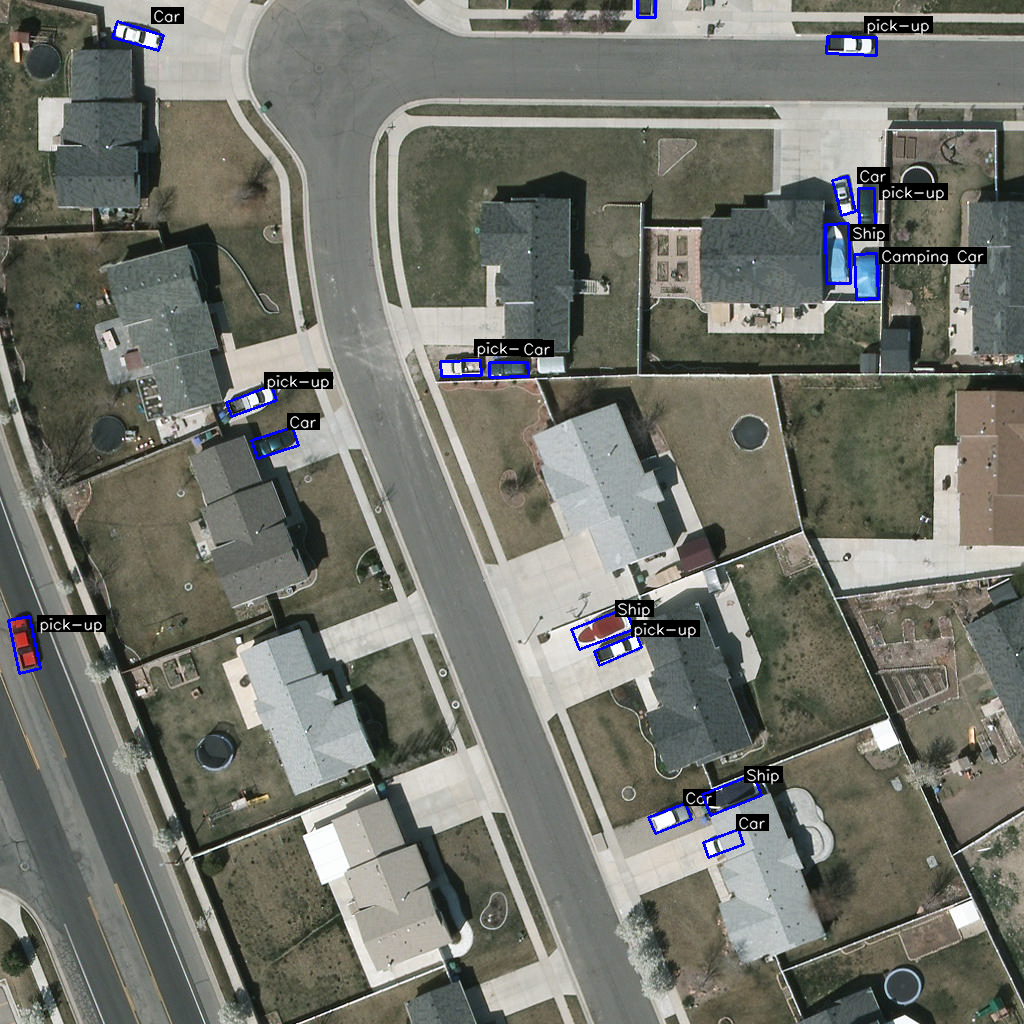
\includegraphics[trim={600pt 1000pt 350pt 0pt},clip,width=\textwidth]{images/bb_smaller0.png}
        \caption{Two Coordinate out of range and smaller 0}
        \label{fig:smaller0}
    \end{subfigure}
    \hfill
    \begin{subfigure}[b]{0.45\textwidth}
        \centering
        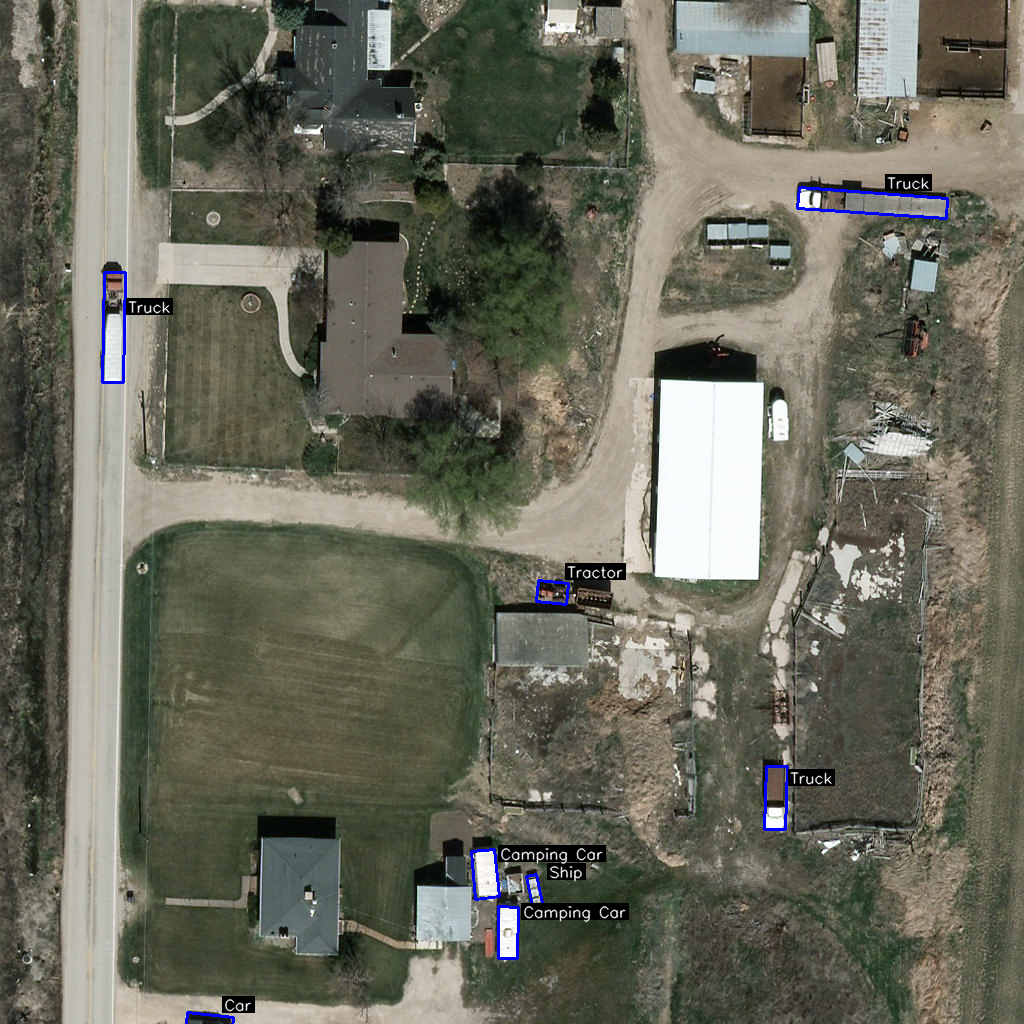
\includegraphics[trim={180pt 0pt 750pt 993pt},clip,width=\textwidth]{images/bb_higher1.png}
        \caption{Two Coordinates out ouf range and higher 1}
        \label{fig:higher1}
    \end{subfigure}
    \caption[Example for label coordinates outside of the image]{Example for label coordinates outside of the image (for full-sized Image see \ref{fig:example_coords_ooR_fs})}
    \label{fig:example_coords_ooR}
\end{figure}

Da die von \citeauthor{Razakarivony2015} \cite{Razakarivony2015} verwendeten Folds nicht disjunkt waren, erhöhte sich das Risiko von Overfitting (s. Kap. \ref{subsec:overfitting}), sodass eigene Folds erstellt werden mussten, deren Erstellung im folgenden Kapitel beschrieben wird. \todo{satz überarbeitne, doppelung}






\section{6-Fold-Cross-Validation}
\label{sec_5Fold_CV}
\todo{es ist eigentlich 6 fold cross validation}

Um die Robustheit der Ergebnisse sicherzustellen und eine fundierte Vergleichbarkeit verschiedener Modelle zu ermöglichen, wurde in dieser Arbeit eine 6-Fold-Cross-Validation angewendet. Insbesondere wurde Wert darauf gelegt, die Evaluation nicht nur auf einem Teildatensatz durchzuführen, sondern eine Mehrfachteilung der Daten vorzunehmen, sodass Schwankungen durch unterschiedliche Trainings- und Validierungsaufteilungen minimiert werden.

Im Gegensatz zu den von \citeauthor{Razakarivony2015} \cite{Razakarivony2015} bereitgestellten Folds, deren Zusammenstellung identische Bilder gleichzeitig im Trainings- und Validierungssatz aufweist, wurden für diese Arbeit eigene, disjunkte Folds generiert. Letztere gewährleisten, dass keine Überlappungen zwischen Trainings- und Validierungsdaten existieren und somit die Gefahr von verfälschten Trainingsergebnissen durch Overfitting ausgeschlossen ist. Die genaue Methodik der Fold-Erstellung ist in Kapitel \ref{subsec:Fold_creation} beschrieben. \todo{absatz überarbeiten wiederholung mit 4.5}

Die Datenaufteilung erfolgte in sechs Folds (0-5): Fünf Folds (Fold 0 bis 4) wurden jeweils für Training und Validierung genutzt, während Fold 5 ausschließlich für abschließende Testzwecke reserviert blieb. Dadurch wurde erreicht, dass die finale Evaluation auf bisher ungesehenen, neutralen Daten stattfand.

Ein besonderes Augenmerk galt einer homogenen Verteilung der Objekte und Objektklassen über alle Folds hinweg. Jeder Fold umfasst zwischen 207 und 221 Bilder, darin enthalten sind jeweils drei bis sieben reine Hintergrundbilder ohne Objekte. Dies ermöglichte eine ausgewogene und repräsentative Bewertung der Modelle hinsichtlich aller vorkommenden Klassen. Die resultierende Klassen- und Bildverteilung pro Fold ist in Tabelle~\ref{tab:fold_distribution} dargestellt.

Insgesamt trägt dieses Verfahren dazu bei, dass die experimentellen Resultate eine hohe Validität aufweisen und zuverlässig Rückschlüsse auf die Auswirkungen der zusätzlichen Kanäle bei den verwendeten Modelle erlauben.


\begin{table}[h!]
\centering
\begin{tabular}{lcccccc}
\textbf{Class/Fold} & \textit{0} & \textit{1} & \textit{2} & \textit{3} & \textit{4} & \textit{5} \\
\hline
\textit{Car}              & 229 & 239 & 226 & 225 & 240 & 225 \\
\textit{Truck}            & 51  & 57  & 50  & 49  & 51  & 50  \\
\textit{Ship}             & 30  & 28  & 29  & 30  & 27  & 27  \\
\textit{Tractor}          & 30  & 32  & 33  & 30  & 31  & 30  \\
\textit{Camping car}      & 65  & 72  & 64  & 69  & 64  & 63  \\
\textit{Van}              & 18  & 17  & 17  & 17  & 16  & 16  \\
\textit{Vehicle}          & 34  & 37  & 34  & 34  & 39  & 33  \\
\textit{Pick-Up}          & 164 & 161 & 157 & 160 & 159 & 157 \\
\textit{Plane}            & 4   & 11  & 4   & 18  & 4   & 7   \\
\textit{Quantity Images}  & 206 & 214 & 221 & 211 & 207 & 209 \\
\textit{Background Images}& 7   & 3   & 3   & 3   & 3   & 3   \\
\hline
\end{tabular}
\caption{Class distribution across folds.}
\label{tab:fold_distribution}
\end{table}
% \begin{itemize}
%         \item Cross validation to ensure robustness and better comparison of different models
%         \item create own folds, as the ones provided by the paper had the same images in training and validation data
%         \item  6 Folds
%         \item 5 for Training and Validation, 1 for Test (Fold 5)
%         \item Good object distribution between the folds
%         \item 207-221 Images per Fold, where 3 or 7 Images are only background
        
%         \item Methodik wurde in Sec. \ref{subsec:Fold_creation} beschrieben
%         \item \todo{Tabelle mit Verteilung einfügen}
%         \item Sagen das die ursprünglichen Fodls des VEDAI Datasets nicht disjunkt sind -> Trainingsergebnisse verfälscht, deshalb eigene Folds erstellt
%     \end{itemize}


% \subsection{YOLOv9u}
% \begin{itemize}
%     \item Implementierung von YOLOv9 auf Basis von YOLOv8.1.23 \cite{yolo_v9u_github}
%     \item erweiterung von yolov9 mit object detection, instance segmentation, oriented object detection, pose estimation, image classficitation, transformer-based object detection \cite{wang2024yolov9}
% \end{itemize}
% \subsection{YOLOv9e}
% \begin{itemize}
%     \item yolov9 Modelle reichen von der t variante mit (imgsize: 640, flops 7.7) bis zur e variante mit (192,5 gflops)
%     \item aufgrund der besten genauigketi und der höchsten flop rate wird das yolov9e modell bei den axis aligend bounding boxen genutzt
% \end{itemize}
% \subsection{Hyperparameter}
% \todo{wird bei Implementierung beschrieben, hier raus nehmen?}


% \begin{itemize}
%     \item DOTA bietet sich als pretrained Model Datengrundlage für die Permutationsexperimente an, da es viele verschieden Klassen auf Satellitenbildern enthält
%     \item Bildgröße von 800 \texttimes 800 bis 20.000 \texttimes 20.000 Pixel
%     \item 3 Channel (Red, Green, Blue) und Grayscale Images (Panchromatic Band von GF2 und JL1 Satelliten)
%     \item Satellite Images von Google Earth und anderne Quellen
%     \item \todo{Bsp. Bild für jede Klasse zeigen (aus Paper nehmen!; Quellenverlinkung für text und bild nicht vergessen); habe alle 16 Klassen für das Training genutzt, wichtig sind trotzdem nur Large Vehicle, Plane, Ship, small vehicle}
% \end{itemize}


\section{High-Performance-Cluster PALMA}

Für das Training der Modelle wurde das \acrfull{HPC} \Acrshort{PALMA} der Universität Münster genutzt. Als Arbeitsumgebung kam dabei eine isolierte \texttt{Python}-Umgebung (UV \cite{palma_uv}) zum Einsatz. Die Ausführung der Trainingsprozesse erfolgte über selbst entwickelte \texttt{Bash}-Skripte, die auf unterschiedlichen \acrshort{GPU}-Knoten des Clusters (u.\,a. HGX-Knoten) verteilt wurden, um eine effiziente Parallelisierung der Trainings zu ermöglichen.

PALMA (Abkürzung für "\Acrlong{PALMA}") wird von dem \Acrfull{CIT} der Universität Münster, basierend auf Hardware der Firma MEGWARE, bereitgestellt \cite{palma_spec} und verfügt über die in Tab. \ref{tab:Spec_Palma} technische Spezifikationen \cite{palma_spec}:



\begin{table}[h!]
\centering
\begin{tabular}{ll}
\multicolumn{2}{c}{\textbf{Palma Specifications}} \\ \hline
\textbf{Total number of \acrshort{CPU} cores} & 16,272 \\
\textbf{Memory} & 77,568\,\acrshort{GB} \\
\textbf{Number of compute nodes} & 444 \\
\textbf{Processor} & Intel Xeon Gold 6140 (18~cores, 2.30\,\acrshort{GHz}, Skylake architecture) \\
\textbf{Network interconnect} & 100\,\acrshort{GHz}/s Intel Omni-Path \\
\textbf{Storage system} & \acrshort{GPFS} with a total capacity of 2.4\,\acrshort{PB} \\
\textbf{Linpack performance} & \textit{R\textsubscript{max}} = 800\,\acrshort{TFLOP}/s; \textit{R\textsubscript{peak}} = 1,277\,\acrshort{TFLOP}/s \\
\textbf{Operating system} & Rocky Linux 9 \\
\hline
\end{tabular}
\caption{System overview PALMA}
\label{tab:Spec_Palma}
\end{table}

Die hohe Rechenleistung und Speicherkapazität des Clusters machten es möglich, auch komplexe Trainingsprozesse mit vielen hochauflösenden Bilddaten effizient und schnell zu verarbeiten.
% \begin{itemize}
%     \item UV als Python Umgebung auf Palma genutzt
%     \item Bash Scripte geschrieben um die Modelle auf diversen GPUS (HGX, etc) zu trainieren
% \end{itemize}
% \begin{itemize}
%     \item Hersteller: MEGWARE\cite{palma_spec}
%     \item 16.272 Cores
%     \item 77.568 GB Memory
%     \item 444 Nodes
%     \item Processor: Intel Xeon Gold 6140 18C @ 2.30GHz (Skylake)
%     \item Interconnect 100Gbit/s Intel Omni-Path
%     \item GPFS Storage: 2,4 PB
%     \item Linpack Performance: Rmax: 800 TFlop/sRpeak: 1,277 TFlop/s
%     \item OS: Rocky Linux 9 
% \end{itemize}

% \subsection{Challenges Preprocessing}
% \subsubsection{VEDAI Dataset Challenges}
% \begin{itemize}
%     \item Label müssen in yolov9 obb format konvertiert werden
%     \item kleine Anzahl (7/3757) war kleiner als 0 oder größer als 1
%     \item Lösung mit Exception Handling und Runden der Werte
%     \item \todo{Beispielbilder einfügen}
% \end{itemize}

% \section{Workflow}
% \subsection{Axis Aligned vs. Oriented Bounding Boxes}
% \begin{itemize}
%     \item Vergleich zwischen Axis Aligned udn Oriented Bounding Boxen
%     \item YOLOv9 arbeitet ursprünglich nur mit aab Boxen
%     \item YOLOv9u kann mit obb arbeiten, da Codebasis von YOLOv8 von Ultralytics, was obb unterstützt
%     \item 
% \end{itemize}
% \begin{itemize}
%     \item \todo{Vergleichsbilder (Schiff und Auto Vergleich) einfügen}
%     \item mehr Blankspace bei axis aligned Bbs
%     \item Concentration of the box on the actual object, significantly less surrounding area outlined. No overlap between bounding boxes (Bei Ship bb)
%     \item 
% \end{itemize}
% \subsection{Channel Permutation}
% \begin{itemize}
%     \item Folgende Permutation werden im Rahmen der Arbeit evaluiert: RGBIR, IRGB, RIRB; RGB, RGIR, RGBNDVI, GBNDBVI
% \end{itemize}
% \subsection{DOTA Training}
% \begin{itemize}
%     \item DOTA als Pretrained Modell für Channel Permutation, map50-95 around 0.4 and training over around 800 epcohs 
%     \item \todo{Result.png einfügen? oder doch sein lassen?}
% \end{itemize}
% \subsection{Ablation Studie}
% \begin{itemize}
%     \item Ablation Study für R, G, B, IR, NDVI durchgeführt
% \end{itemize}


\section{Bash Scripts}

Für das Training der Modelle wurden mehrere \texttt{Bash}-Skripte entwickelt, die für den Hochleistungsrechner \acrshort{PALMA} ausgelegt waren. Die Trainingsläufe erfolgten primär über \texttt{\acrshort{SLURM} Job Arrays}, wobei jeder Fold einer Permutation einem separaten Job zugeordnet wurde. Somit entsprach ein Modell stets einem Fold innerhalb einer bestimmten Permutation.  

Die Entscheidung zwischen \acrlong{abb} und \acrlong{obb} erfolgte unter denselben Trainingsparametern wie bei den Permutationsexperimenten (s. Tab.~\ref{tab:hyperparameters}), jedoch mit unterschiedlichen Modellen: \texttt{YOLOv9e} für \acrshort{abb} und \texttt{YOLOv9u} für \acrshort{obb}, da jeweils nur diese Varianten die entsprechenden Bounding-Box-Formate unterstützen. In diesem Fall wurde kein vortrainiertes Modell genutzt, sondern ein Training \textit{from scratch} durchgeführt.  

Im Anschluss wurden die Permutationsexperimente durchgeführt. Dabei kamen einheitlich die in Tab.~\ref{tab:hyperparameters} aufgeführten Hyperparameter zum Einsatz. Die Bildauflösung betrug 1024~$\times$~1024 Pixel, die Trainingsdauer umfasste 500 Epochen, und ein frühzeitiges Beenden war durch einen \texttt{patience}-Wert von 0 deaktiviert, um eine konsistente Vergleichbarkeit sicherzustellen. Grundlage war ein auf dem \acrshort{DOTA}-Datensatz vortrainiertes Modell, wobei durchgängig die Architektur \texttt{YOLOv9u} (s. Kap.~\ref{subsec:yolov9u}) verwendet wurde.  

Für die Ablationsstudien wurde hingegen auf den Einsatz eines vortrainierten Modells verzichtet, während alle übrigen Trainingsparameter unverändert blieben.  

Nach Abschluss des Trainings wurde jeweils das Modell mit der besten Validierungsleistung ausgewählt und anschließend auf den entsprechenden Testfold angewendet. Die Evaluation erfolgte in beiden Fällen in einem einmaligen Durchlauf, um konsistente und vergleichbare Ergebnisse zu gewährleisten.  


% Für das Training der Modelle wurden mehrere \texttt{Bash}-Skripte entwickelt, die für den Einsatz auf dem Hochleistungsrechner \acrshort{PALMA} konzipiert wurden. Die Trainingsläufe wurden primär mittels \texttt{\acrshort{SLURM} Job Arrays} durchgeführt, wobei jeder Fold einer Permutation einem eigenen Job zugewiesen wurde. Somit entsprach ein Modell jeweils einem Fold innerhalb einer bestimmten Permutation.

% Für die Entscheidung zwischen \Acrlong{abb} und \Acrlong{obb} wurden die gleichen Trainingsparameter wie bei den Permutationsexperimenten (s. Tab. \ref{tab:hyperparameters}), aber verschiedene Modelle genutzt. YOLOv9e wurde für die \acrshort{abb} Boxen genutzt und YOLOv9u für die \acrshort{obb} Boxen eingesetzt, da nur jeweils diese Modelle die verschiedenen Bounding Box Arten unterstützen. Es wurde kein vortrainiertes Modell verwendet, sondern von Scratch trainiert.

% Im Rahmen des Permutationstrainings kamen für sämtliche Permutationen einheitlich die in Tabelle \ref{tab:hyperparameters} aufgeführten Hyperparameter zum Einsatz. 
% Die Bildauflösung betrug 1024~$\times$~1024 Pixel, die Trainingsdauer umfasste 500 Epochen, und das frühzeitige Beenden des Trainings war durch einen \texttt{patience}-Wert von 0 deaktiviert, um eine konsistente Vergleichbarkeit zu gewährleisten. 

% Verwendet wurde ein vortrainiertes Modell auf dem \acrshort{DOTA}-Datensatz (s. Chap. \ref{subsec:DOTA}), wobei die Modellarchitektur \texttt{YOLOv9u} (s. Chap. \ref{subsec:yolov9u}) durchgängig zum Einsatz kam.

% Für die Ablationsstudien wurde auf den Einsatz des vortrainierten Modelles verzichtet; alle übrigen Trainingsparameter blieben unverändert.

% Nach Abschluss des Trainings wurde jeweils das Modell mit der besten Leistung auf den Validierungsdaten evaluiert. Anschließend erfolgte die Anwendung dieses Modells auf dem entsprechenden Testfold. In beiden Fällen wurde die Evaluation in einem einmaligen Durchlauf durchgeführt, um konsistente und vergleichbare Ergebnisse zu gewährleisten.

\begin{table}[htbp]
\centering
\caption{Key training hyperparameters at the \acrshort{RGB} Permutation (Fold 4)}
\label{tab:hyperparameters}
\begin{tabular}{ll}
\hline
\textbf{Hyperparameter} & \textbf{Value / Description} \\
\hline
Task & Oriented Bounding Box (OBB) \\
Mode & Training \\
Model & YOLOv9u, pretrained on \acrshort{DOTA} \\
Dataset & \acrshort{VEDAI}  \\
Epochs & 500 \\
Batch size & 4 \\
Image size & 1024 × 1024 px \\
Early stopping (patience) & 0 (disabled) \\
Optimizer & Auto \\
Initial learning rate ($lr_0$) & 0.01 \\
Momentum & 0.937 \\
Weight decay & 0.0005 \\
Warmup epochs & 3 \\
Data augmentation & FlipLR 0.5, Mosaic 1.0, Erasing 0.4, AutoAugment randaugment \\
Device & GPUs 0,1,2,3 \\
Workers & 8 \\
Save directory & \texttt{/scratch/tmp/t\_liet02/cross\_validation/rgb/fold4} \\
\hline
\end{tabular}
\end{table}

% \begin{itemize}
%     \item Diverse Bash Scripte für PALMA geschriebne um die Modelle zu trainieren. 
%     \item Hauptsächlich SLURM Job Arrays genutzt um jeweils alle Folds einer Permutation durchlaufen (jeder Fold einer Permutation bekommt einen Job = ein modell)
%     \item hyperparameter (für permutation training): imagesize:1024; epochs: 500, patience: 0 (ausgestellt um zur besseren Vergleichbarkeit alle Modelle immer exakt 500 epochs durchzutrainieren); pretrained true (dota dataset,  ref zu beschreibung einfügen); als modell immer yolov9u (ref einfügen)
%     \item für ablation training: kein pretrained model, sonst alles gleich
%     \item danach immer validierung des besten val modells auf den val daten 
%     \item dann das beste validierungsmodell auf dem testfold
%     \item beides mal nur ein durchlauf daten zur evaluation zu erhalten
% \end{itemize}


